Una volta isolati i segmenti di iride d’interesse dall’immagine originale si può procedere all’ultima fase di questa sezione di elaborazione delle immagini. Come si è visto prima, la fase di segmentazione produce un’immagine completamente a sfondo nero tranne nella parte in cui è presente la regione di interesse. L’elevata presenza di pixel neri, i quali non contengono informazioni utili,  potrebbe “confondere” la rete neurale, la quale darebbe pesi errati alle sezioni nere. Risulta quindi necessario ritagliare l’immagine in modo tale da valorizzare al massimo i pixel effettivamente utili, ovvero quelli del segmento. Tale operazione si chiama cropping e la funzione seguente ne è l’implementazione:

\begin{minted}
  [
    xleftmargin=\parindent,
    framesep=2mm,
    baselinestretch=1.2,  
    fontsize=\footnotesize,
    linenos,
    breaklines
  ]
  {python}
  
  def crop_image(masked_image, offset=30, tollerance=80):
   mask = masked_image > tollerance
   coords = np.argwhere(mask)
   x0, y0 = coords.min(axis=0)
   x1, y1 = coords.max(axis=0) + 1  # slices are exclusive at the top
   cropped = masked_image[x0 - offset: x1 + offset, y0 - offset: y1 + offset]
   return cropped  
\end{minted}

La funzione restringe l’immagine attorno ai pixel non neri, quindi quelli definiti dal segmento di iride, riducendo al minimo possibile il nero senza eliminare i pixel contenenti l’informazione utile.

\begin{figure}[h]
  \centering
  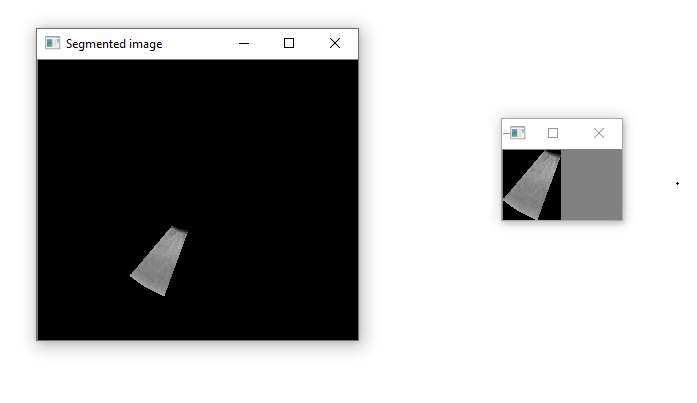
\includegraphics[width=1.0\textwidth]{crop.png}
  \caption{Operazione di cropping dell'immagine}
\end{figure}

Al termine di questo passaggio si ottengono quindi immagini relativamente piccole nel quale la maggior parte dei pixel rappresenta la regione di interesse.

A questo punto il dataset per il training è quasi pronto, tuttavia prima bisogna risolvere un problema introdotto dal cropping. Anche partendo da immagini della stessa dimensione i vari segmenti d’iride possono risultare di dimensione diversa in quanto le naturali conformazioni dell’occhio umano non sono mai perfettamente uguali, quindi il cropping su questi segmenti potrebbe produrre immagini di dimensione diversa. Immagini a dimensione non uniforme non vanno bene per una CNN in quanto nel processo di training essa si aspetta in input matrici (rappresentazione interna delle immagini) tutte della stessa dimensione. Per risolvere questo problema si è implementato un meccanismo di resize automatico delle immagini dei segmenti alla loro dimensione media.

\begin{minted}
  [
    xleftmargin=\parindent,
    framesep=2mm,
    baselinestretch=1.2,  
    fontsize=\footnotesize,
    linenos,
    breaklines
  ]
  {python}
  
  def get_average_shape(cropped_dict):
   shapes = np.concatenate(([c.shape for c in cropped_dict['DB_PROBS']], [c.shape for c in cropped_dict['DB_NORMAL']]))
   means = np.around(np.mean(shapes, axis=0)).astype(int)
   return means 
\end{minted}

Utilizzando la funzione sopra citata si calcolano height e width medie tra tutte le immagini risultanti dalla fase di cropping,  poi si procede, tramite la funzione \texttt{cv2.resize} di OpenCV, al ridimensionamento di tali immagini alle dimensioni trovate. E’ vero che un resize potrebbe portare ad una riduzione della qualità dell’immagine (ad esempio un ingrandimento risulterebbe in un'immagine sgranata) tuttavia le dimensioni ottenute dopo il cropping risultano molto vicine tra di loro quindi un resize alla dimensione media non comporta una grossa perdita di qualità.

A questo punto si è definitivamente pronti per la fase di training; lo script \texttt{preprocess.py} termina con il salvataggio delle immagini croppate e ridimensionate nella cartella \texttt{TEMP\_SEG}; vengono poi suddivise in due sotto cartelle, \texttt{DB\_NORMAL\_SEG} e \texttt{DB\_PROBS\_SEG}, in relazione alla loro sottocartella di \texttt{DATA\_IMAGES} di provenienza.
